% ------------------------------------------------------------------------
% bjourdoc.tex for birkjour.cls*******************************************
% ------------------------------------------------------------------------
%%%%%%%%%%%%%%%%%%%%%%%%%%%%%%%%%%%%%%%%%%%%%%%%%%%%%%%%%%%%%%%%%%%%%%%%%%

\documentclass{birkjour}
%%%Optional but convenient to use is the package ``cite''. If you do not want to use, remark the next line by placing the percent sign % in front of it:
\usepackage[noadjust]{cite}
\usepackage{amsmath}
\usepackage{url}
%
%
% THEOREM Environments (Examples)-----------------------------------------
%
 \newtheorem{thm}{Theorem}[section]
 \newtheorem{cor}[thm]{Corollary}
 \newtheorem{lem}[thm]{Lemma}
 \newtheorem{prop}[thm]{Proposition}
 \theoremstyle{definition}
 \newtheorem{defn}[thm]{Definition}
 \theoremstyle{remark}
 \newtheorem{rem}[thm]{Remark}
\newtheorem{comment}[thm]{Comment}
 \newtheorem*{ex}{Example}
 \numberwithin{equation}{section}

\newcommand{\ed}{\end{document}}
\begin{document}

%-------------------------------------------------------------------------
% editorial commands: to be inserted by the editorial office
%
%\firstpage{1} \volume{228} \Copyrightyear{2004} \DOI{003-0001}
%
%
%\seriesextra{Just an add-on}
%\seriesextraline{This is the Concrete Title of this Book\br H.E. R and S.T.C. W, Eds.}
%
% for journals:
%
%\firstpage{1}
%\issuenumber{1}
%\Volumeandyear{1 (2004)}
%\Copyrightyear{2004}
%\DOI{003-xxxx-y}
%\Signet
%\commby{inhouse}
%\submitted{March 14, 2003}
%\received{March 16, 2000}
%\revised{June 1, 2000}
%\accepted{July 22, 2000}
%
%
%
%---------------------------------------------------------------------------
%Insert here the title, affiliations and abstract:
%


\title[Visually pleasing knot projections]{Visually pleasing knot projections}




%----------Author 1
\author[Hankin]{Robin K. S. Hankin}

\address{%
55 Wellesley Street East, Auckland 1010, New Zealand}

\email{hankin.robin@gmail.com}

%----------classification, keywords, date
\subjclass{Primary 57K10-XX; 32-XX}

\keywords{Knot projections, Bezier curves, Multidimensional optimization}

\date{\today}
%----------additions
%%% ----------------------------------------------------------------------

\begin{abstract}
In this short article I discuss the \ae sthetics of knot projections
and introduce software which creates two dimensional knot diagrams
optimized for visual appearance.  The software is in the form of a
documented and self-contained suite of functionality written in the R
programming language (that is, a ``package"): {\tt knotR}.  The
package leverages the graphical capabilities of the popular vectorized
graphics software {\tt inkscape}.  Different aspects of knot
appearance are discussed and a framework for objectively optimizing
the visual appeal of a knot projection is given.  I use the software
to create a wide range of knot diagrams.
\end{abstract}

%%% ----------------------------------------------------------------------
\maketitle
%%% ----------------------------------------------------------------------
%\tableofcontents

\section{Introduction}

A {\em mathematical knot} is a smooth, unoriented embedding of a
circle~$\mathbb{S}^1$ into~$\mathbb{R}^3$~\cite{manturov2004,adams2004}.  Two
knots are said to be equivalent if the embedding of one can be
continuously deformed to the other; if so, there is a
homeomorphism~$h\colon\mathbb{R}^3\longrightarrow\mathbb{R}^3$ which
takes one embedded circle to the other.  In the art world, knot theory
has applications to the study of dance~\cite{khorami2020}, sculpture,
\cite{bosch2010, widmark2020}, and many other branches of mathematical
art~\cite{hart2008}.

It is common to present a knot using diagrams such as
Figure~\ref{knot_table}, in which a two-dimensional projection of the
knot is given with broken lines indicating where one strand passes
over another.  Knot diagrams have a long history:
Przytycki~\cite{przytycki1998} discusses an intricate braid drawn
around 1700\,BC; they figure prominently in {\em The Book of Kells}
and the Lindisfarne gospels, graphic art produced around
800\,AD~\cite{bain1973}.  Such artwork makes extensive use of
symmetry~\cite{cromwell2008}, and its visual appeal persists to the
present day~\cite{antonsen2021}.  More recent examples would include
bobbin lace~\cite{irvine2020}, in which many threads are braided
together to form a loose fabric.  The enduring popularity of such
fibre arts attests to the aesthetic of knots and braids in the modern
world.

Knot diagrams are ubiquitous in the modern discipline of mathematical
knot theory.  In the nineteenth century we see Tait~\cite{tait1884}
publishing an early systematic study of knots including a beautiful
plate of elegantly hand-drawn cursive knot diagrams.  The tradition
continues into the twentieth century with Rolfsen~\cite{rolfsen1976}
presenting an appendix containing many knot and link projections.
Rolfsen's diagrams are used widely today: Adams~\cite{adams2004}
reproduces his work extensively, as do many more recent works.

\subsection{Computer-generated knot visualisations}

Online resources are becoming more widely available, with one
prominent example being the {\em Knot Atlas}~\cite{knot_atlas}
presenting extensive knot tables following
Rolfsen~\cite{rolfsen1976}---for knots up to~10 crossings---and
Thistlethwaite~\cite{hoste1998}, for knots of~11 crossings.

Symbolic software such as Mathematica and Maple can be used to produce
representations of knots, typically in the form of nonstandard
embeddings of the torus into~$\mathbb{R}^3$; but as discussed below
this approach is suboptimal from the perspective of producing a
visually pleasing projection.

Visual appeal of knot projections appears to be important to
contemporary mathematicians.  Recent work by Taalman (writing as
mathgrrl)~\cite{taalman2019}, for example, shows that large amounts of
effort have been expended by serious mathematicians making
representations of knots attractive.  Bosch~\cite{bosch2010}, taking a
different approach to knot representations, presents artwork that
utilises high-dimensional computer optimization, as here.

No discussion of computer-generated representations of knots would be
complete without mentioning the tour de force that is~{\em
  KnotPlot}~\cite{scharein1997,scharein1998} which includes extensive
functionality for visualising knots.  Much of the visualization
considers (nonstandard) embeddings of a torus in $\mathbb{R}^3$; the
configuration is ``relaxed'' in such a way as to produce a smoother
output.  {\em KnotPlot} has two major display modes: any knot may be
displayed in either a ``beads and sticks" mode or in a ``smooth tubes"
mode.  The software does render knot diagrams but the author states
[p77] that ``knots with higher crossing numbers (greater than six or
seven) will not produce good 2D projections when fully relaxed", and
admits that some of the diagrams are ``a bit messy".

%One of the early works using this approach is the 1932 German classic
%Anschauliche Geometrie by David Hilbert and S. Cohn-Vossen, available
%in English translation as Geometry and the Imagination [HCV52].  This
%book is remarkable for the quality of insight and also for its
%incredible diagrams, mostly hand drawn and (obviously) predating the
%computer era.

\subsubsection{Knot theory in R}

The R programming language~\cite{rcore2021}, while usually associated
with statistical analysis and data processing, is also a suitable tool
for producing visually attractive images.  Generative art [that is,
  use of an algorithm, with or without a random component, in a
  creative process] is possible in R~\cite{brunner2021}.  More
specifically to knot theory, the {\tt Rknots}
package\cite{comoglio2011,comoglio2016} presents software for folded
protein structures, and includes 3D renderings of commonly encountered
knotted strands.

\subsection{Visual knot diagrams: summary}

Two key questions emerge.  Firstly, {\em What makes a knot plot
  attractive?}, and secondly, {\em How best to create knot plots with
  the desired qualities?}  I address both questions, and attempt to
capture the aesthetics of knot diagrams using mathematical
formulations.  These formulations are of two types: hard constraints
of different forms of symmetry; and quantification of various
undesirable qualities of a knot diagram that may be minimized
numerically.  I present software and workflows that not only produce
pleasing knot diagrams, but also allow one to investigate the
connection between the aesthetics of knot diagrams and their
mathematics.

\section{The knotR package: Rationale}

\begin{figure}[h]
  \centering
  \includegraphics[width=10cm]{"1280px-Knot_table".png}  % canonical version in vignettes/ directory
  \caption{A table of prime knots up \label{knot_table} to seven
    crossings, labels following~\cite{alexander1926}.  Image taken
    from~\cite{wikipedia_knot_theory}.}
\end{figure}

Consider Figure~\ref{knot_table} from an \ae sthetic perspective; the
diagrams are representative of those available under a free license.
However, these diagrams are not suitable for high-quality artwork such
as posters: they are not vectorized.  Many of the underlying knots
possess mirror symmetry (at least, the diagrams do if the breaks
are ignored), which is not present in the visual representation.
Also, several of the strands cross at acute angles.  The diagram for
knot~$7_3$, for example, contains kinks and abrupt changes of
curvature which distract from the underlying topological form.

Such considerations suggest that knot diagrams might be produced by
minimization of some objective function that quantifies the visual
inelegance of a knot diagram.  The precise nature of such an objective
function is, of course, a subjective choice but one might require the
following desiderata:

\begin{itemize}
\item Curvature to be as smoothly changing as possible, with limited maximal curvature
\item Strands to cross at right angles
\item Crossing points to be separate from one another
\item Any symmetry desired in the knot should be enforced exactly, and be visually apparent
\end{itemize}

Knot diagrams may be created using vectorized graphics software such
as inkscape~\cite{Inkscape}: one specifies a sequence of control
points, then interpolates between these points to create a knot
diagram with the appropriate topology (inkscape is a widely-used
system available under the GPL).  One way of smoothly interpolating
between specified points is Bezier curves~\cite{olsen2014}.  A Bezier
curve is a visually pleasing polynomial path that can be used to
specify the path of a knot projection; here cubic Bezier curves are
used.  This gives users a convenient, direct control of where these
curve segments will appear; compare G2-continuous B-splines, which
only approximate their control points.

Bezier curves are a natural choice for working with
mathematical knots for several reasons: they are familiar to many
graphical workers; they have a natural and intuitive control system
(usually called ``handles''), and are implemented in many graphical
software suites.  The software discussed here~\cite{hankin2020} allows
one to specify a knot in terms of its Bezier control points within
inkscape, import the object into R~\cite{rcore2021}, and then to use
numerical optimization techniques to improve the visual appearance of
the knot.

One plausible technique for creating knot projections is to consider a
two-dimensional projection of a knot's embedding
$\mathbb{E}\subset\mathbb{R}^3$.  However, this approach often results in
poor visual appearance: cusps or other displeasing effects can occur.

\section{The package in use}

The software presented here is written in the ``R'' programming
language~\cite{rcore2021}, which is usually associated with
statistical analysis and data processing.  However, R possesses a
number of features such as object-oriented programming and
high-dimensional optimization which make it suitable for producing
knot diagrams.  In this section, I give workflows for creating two
simple knots: firstly~$7_6$, followed by the figure-of-eight
knot~$4_1$ which requires imposition of symmetry constraints.

The first step is to create a closed curve in inkscape that shows the
rough outline of the knot~(Figure~\ref{screenshot_inkscape_7_6} shows
a screenshot of {\tt 7\_6\_first\_draft.svg}, supplied with the
package).  Note that this file contains only the knot {\em path}; the
over and under information is to be added later.  Irvine {\em
  et. al.}~\cite{irvine2020} use the terms {\em drawing} and {\em
  braid word} for analogous concepts in their work on bobbin lace
patterns.

Here, knot paths are required to have Bezier handles that are
symmetrically placed with regard to nodes (this is a user-settable
option in inkscape).  One consequence of this design choice is that
radius of curvature is not matched exactly across a node; the path is
not G2 smooth in CAD terminology.  However, because the optimization
routine ensures that the radius of curvature changes only by a small
amount, visual continuity---in the sense of absence of visible
interruptions to a smoothly evolving strand---is preserved.  At a
crossing point it is important that both the unbroken and broken
strands (designated ``overstrand'' and ``understrand'' respectively)
are smooth.  We would like strand crossing points to be far from
nodes, as this ensures visual continuity of strands at crossing
points, especially the understrand (see Figure~\ref{two_trefoil_knots}
for an example and discussion).

\begin{figure}[h]
  \centering
    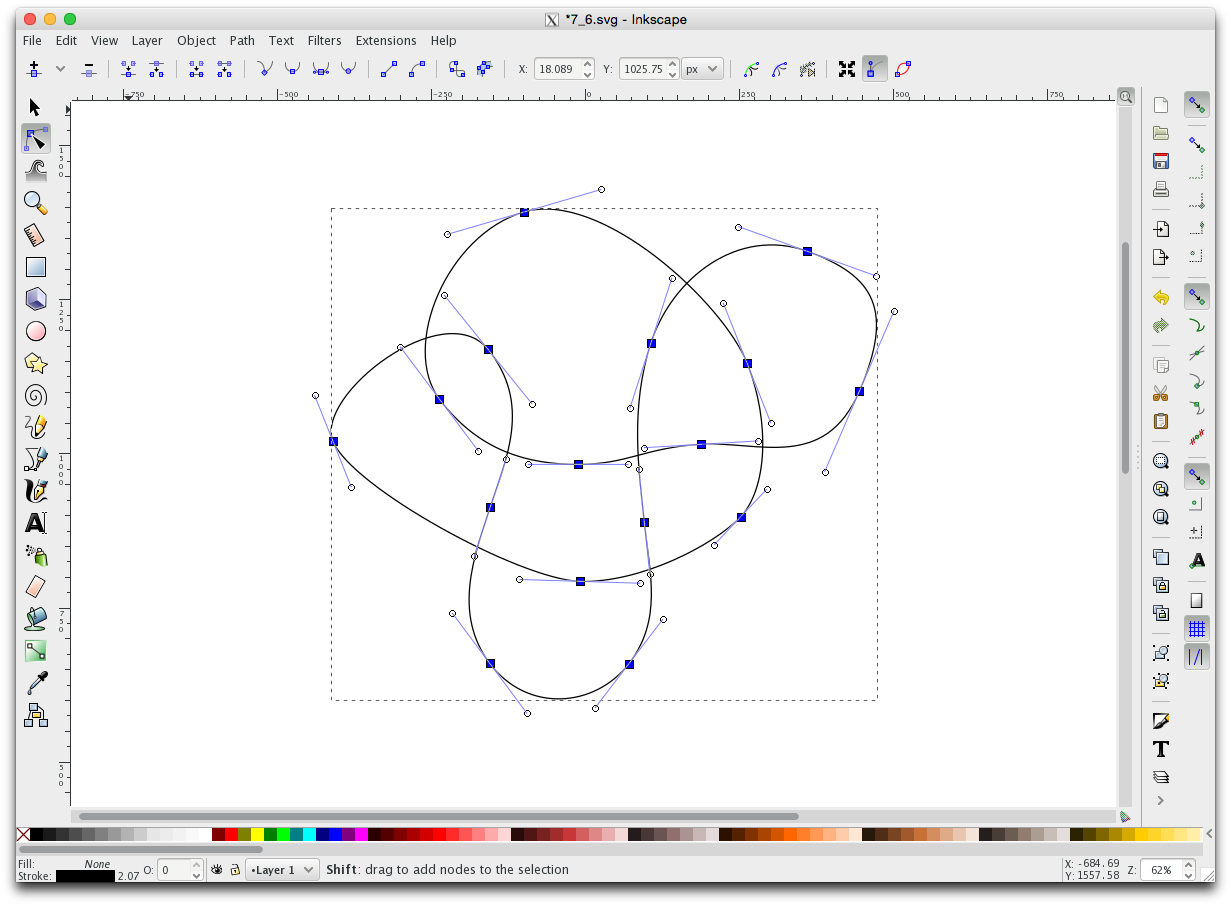
\includegraphics[width=10cm]{screenshot_inkscape_7_6.png} % held in vignettes/ directory
\caption{Screenshot of inkscape\label{screenshot_inkscape_7_6} setup
  for knot~$7_6$.  Nodes are shown as squares, handles as small
  circles, symmetrically placed on either side of nodes}
\end{figure}

The knot shown in Figure~\ref{screenshot_inkscape_7_6} is clearly
suboptimal: even though the nodes are connected by Bezier curves which
are individually smooth, the path as a whole is visually disjointed as
it has places where the radius of curvature changes abruptly.

Although it is possible in principle to improve the visual appearance
of the knot path by hand in inkscape, this is a surprisingly difficult
and frustrating task.  In order to remedy the flaws of the diagram
using an automated system, we first read the {\tt .svg} file into R
using the {\tt reader()} function; a typical R session follows:

\begin{verbatim}
> library(knotR)
> k76 <- reader(system.file("7_6_first_draft.svg",package="knotR"))
> head(k76)

              x         y
[1,]  -98.81963 339.81898
[2,] -223.87754 303.35366
[3,] -299.84521 121.06064
[4,] -236.36319  36.35340
[5,] -172.88118 -48.35384
[6,]  -92.86186 -69.78212
\end{verbatim}

Object~{\tt k76} is stored as an object of class {\tt inkscape}: a
two-column matrix with rows corresponding to the node and handle
positions of the inkscape path.   The object has 49 lines, of which only the  first six are shown.  Inkscape representation has a certain amount of
redundancy as knot paths have handles which are symmetrically placed
with respect to nodes; also, the first node is the same as the last
for the loop is closed.  The package can coerce inkscape objects to
other forms, specifically {\tt minobj} objects, which contain no
redundancy (the position of each node, as well as one of the handles,
is stored); or {\tt controlpoints} objects, which allow for easy
construction of Bezier interpolation between nodes.  Note that increasing the number of nodes provides more control over the path at the expense of a more difficult optimization process.

\begin{figure}[htbp]
  \begin{center}
\begin{verbatim}
> k76_rough <- reader(system.file("7_6_first_draft.svg",package="knotR"))
> knotplot2(k76_rough, seg=TRUE)
\end{verbatim}

\begin{centering}
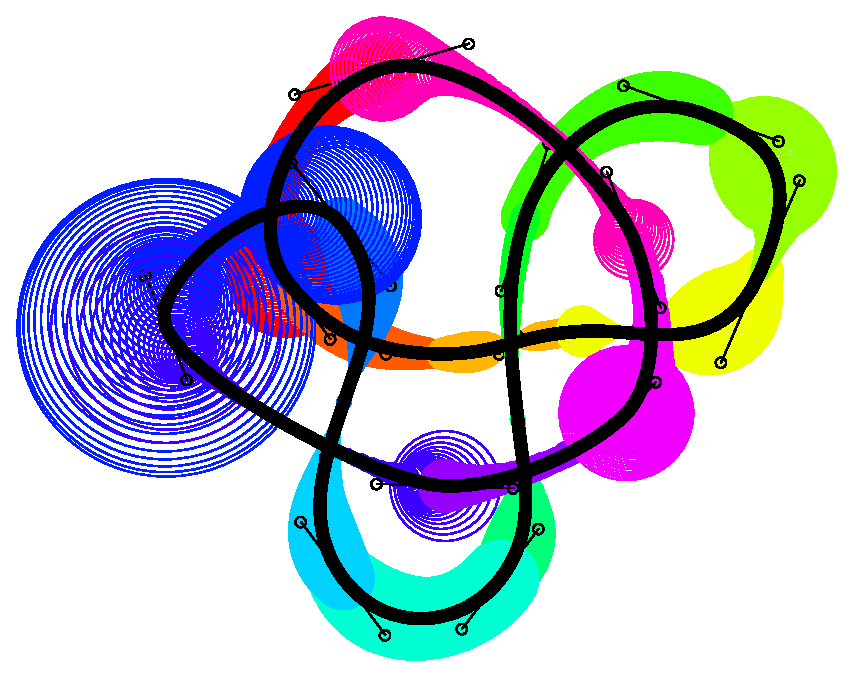
\includegraphics[scale = 0.9]{knot-7_6_rough}
\caption{The \emph{path} of (unoptimized) \label{7_6_rough}
  knot~$7_6$, showing Bezier handles as thin straight lines and
  circles.  The coloured circles have a radius proportional to the
  curvature (that is, the reciprocal of the radius of curvature) along
  the strand.  Colouring is arbitrary, one color for each Bezier
  segment; solid blotches result from densely overlapping circles.
  Note large curvature at loop on left}
  \end{centering}
  \end{center}
\end{figure}

\begin{figure}[!tbp]
\begin{verbatim}
knotplot2(k7_6,text=TRUE,lwd=1,circ=0,rainbow=TRUE)
\end{verbatim}
 \centering
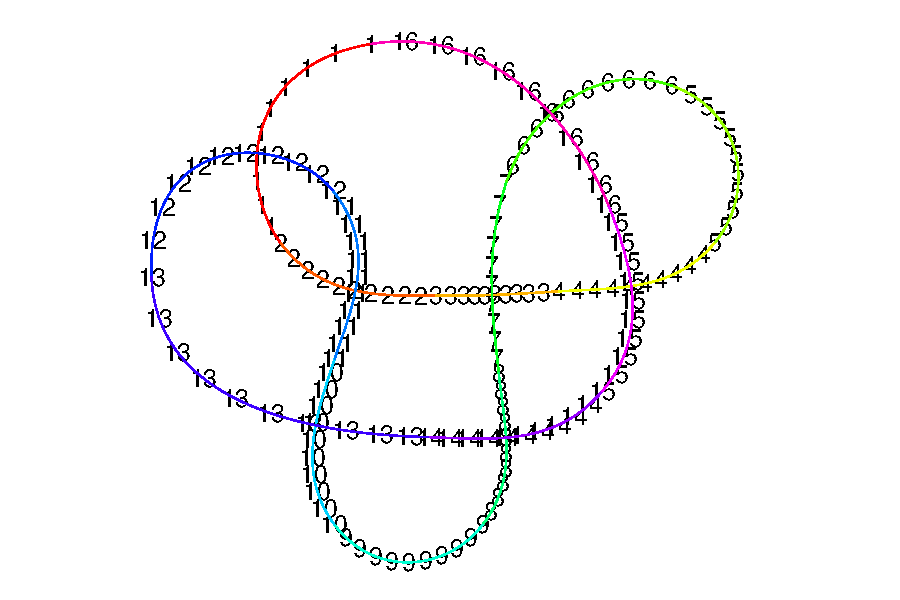
\includegraphics[scale = 0.9]{knot-004}
\caption{Knot~$7_6$ with strands numbered \label{k76_strands} so that
  the sense of the crossings can be established.  For example, strand
  7 should pass over strand 3 as per the {\tt overunder}
  specification.  Crossings become relevant only for the final
  rendering of the knot curve with the gaps included}
\end{figure}

To beautify it we need to specify a function of the path that
quantifies its displeasingness, and then minimize this objective
function using numerical methods.  In the package, minimization is
performed using either Nelder-Mead~\cite{nelder1965} or a Newton-type
method~\cite{dennis1983} (gradient information is not available).  The
optimization proceeds over $\mathbb{R}^n$ where $n$ is the number of
parameters needed to specify the path; typically $n\gtrsim 50$ for the
knots presented here.  In the context of the package, the methods
appear to be broadly comparable.

Two examples of desiderata for such an objective function might be to
keep the strands crossing at right angles, and minimizing overall bending
energy.  These are evaluated in the package by functions
{\tt total\_crossing\_angles()} and~{\tt total\_bending\_energy()}
respectively:

\begin{verbatim}
> b <- as.controlpoints(k76_rough)
> total_crossing_angles(b)

[1] 0.3145033

> total_bending_energy(b)

[1] 0.1276257
\end{verbatim}

The knots supplied in the package minimize a weighted sum of these and
other badnesses\footnote{Function {\tt badness()} includes various
``housekeeping'' badnesses which are used to make sure that the
minimum found by {\tt nlm()} is topologically identical to the
starting configuration (a list is given in the Appendix).  Function
{\tt non\_crossing\_strand\_close\_approach\_badness()}, for example,
makes non-crossing strands ``repel'' one another so as not to
introduce spurious intersections.}.  The weightings for the various
badnesses are, of course, subjective; but the system discussed here
allows the user to change the weightings used and compare results.  I
present a short discussion in section~\ref{section_cca} below.
Numerically, the badnesses are evaluated by function {\tt badness()}:

\begin{verbatim}
> badness(k76_rough)

[1] 6.16279
\end{verbatim}

This function may be minimized by numerical optimization:

\begin{verbatim}
> o <- nlm(badness, as.knotvec(k76_rough))
> k7_6 <- as.minobj(o$estimate)
> badness(k7_6)

  [1] 3.550152
\end{verbatim}

(the above takes about an hour of CPU time: it is optimizing a
function of~64 real variables, and the objective function takes a few
seconds to evaluate).  However, the result is visually smoother and
thus arguably more attractive (Figure~\ref{7_6}).

\begin{figure}[!tbp]
\begin{verbatim}
knotplot2(k7_6)
\end{verbatim}
  \centering
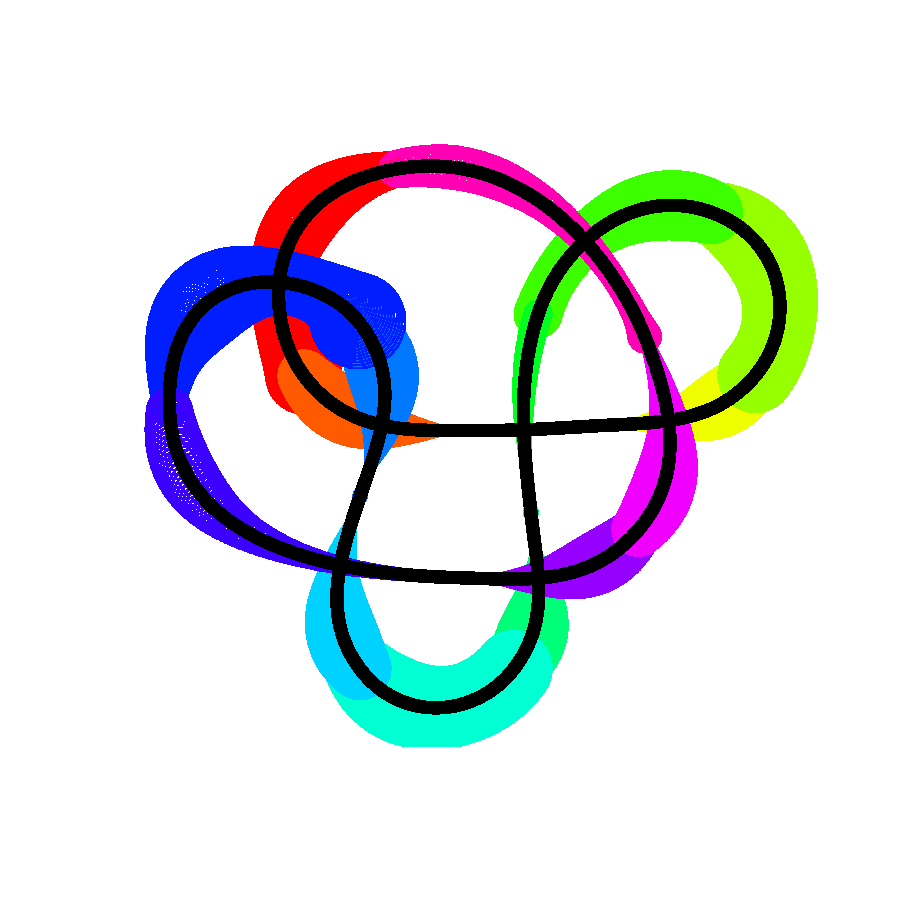
\includegraphics[scale = 0.9]{knot-k76_knotplot2} % in vignettes/ directory
\caption{Knot $7_6$, post-optimization\label{7_6}}
\end{figure}
   
To specify the senses of the knot's\ %---------------------------------'
crossings, we create an overunder object which is a two-column matrix:

\begin{verbatim}
> ou76 <- matrix(c(
+     12,01,
+     02,11,
+     07,03,
+     04,15,
+     16,06,
+     14,08,
+     10,13
+     ),byrow=TRUE,ncol=2)
\end{verbatim}

With reference to Figure~\ref{k76_strands}, each row of {\tt ou76}
corresponds to a crossing; the first element gives the overstrand and
the second the understrand; thus strand~12 passes over strand~1,
strand~2 passes over strand~11, and so on.  The graphical
implementation is indicated in
Figure~\ref{overundergraphicalimplementation}, and the complete knot
is shown in figure~\ref{76_overunder}.

  
\begin{figure}[!tbp] % file overundergraphicalimplementation.pdf is
                     % created in file inst/overunder.R
  \centering
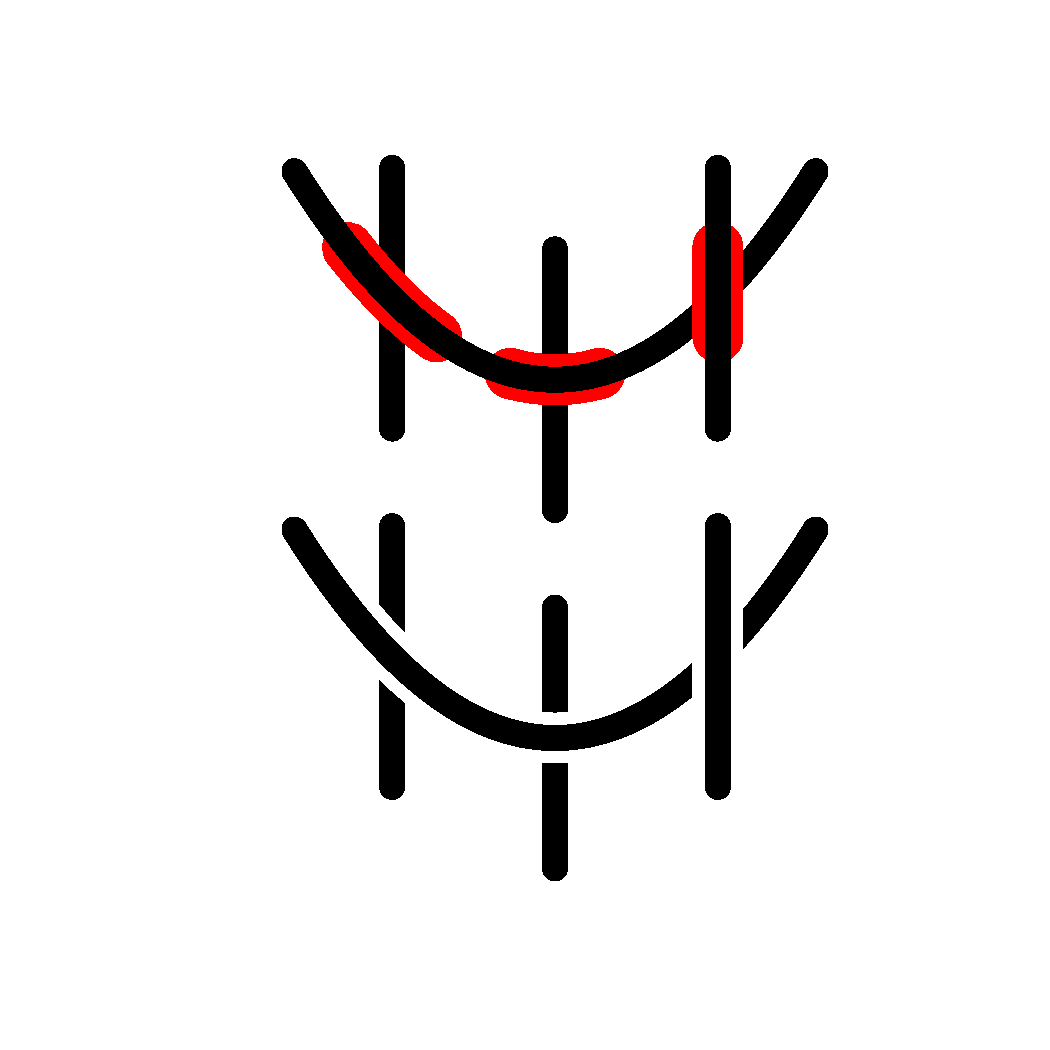
\includegraphics[width=4in]{overundergraphicalimplementation}
\caption{Diagram \label{overundergraphicalimplementation} showing the
  graphical implementation of the line breaks distinguishing
  overstrand from understrand at a crossing point.  Top, details of
  technique used, with mask coloured red.  Bottom, same diagram but
  with mask coloured white, illustrating mechanism for production of
  publication-quality knots}
\end{figure}

\begin{figure}[!tbp]
\begin{verbatim}
knotplot(k7_6)
\end{verbatim}
  \centering
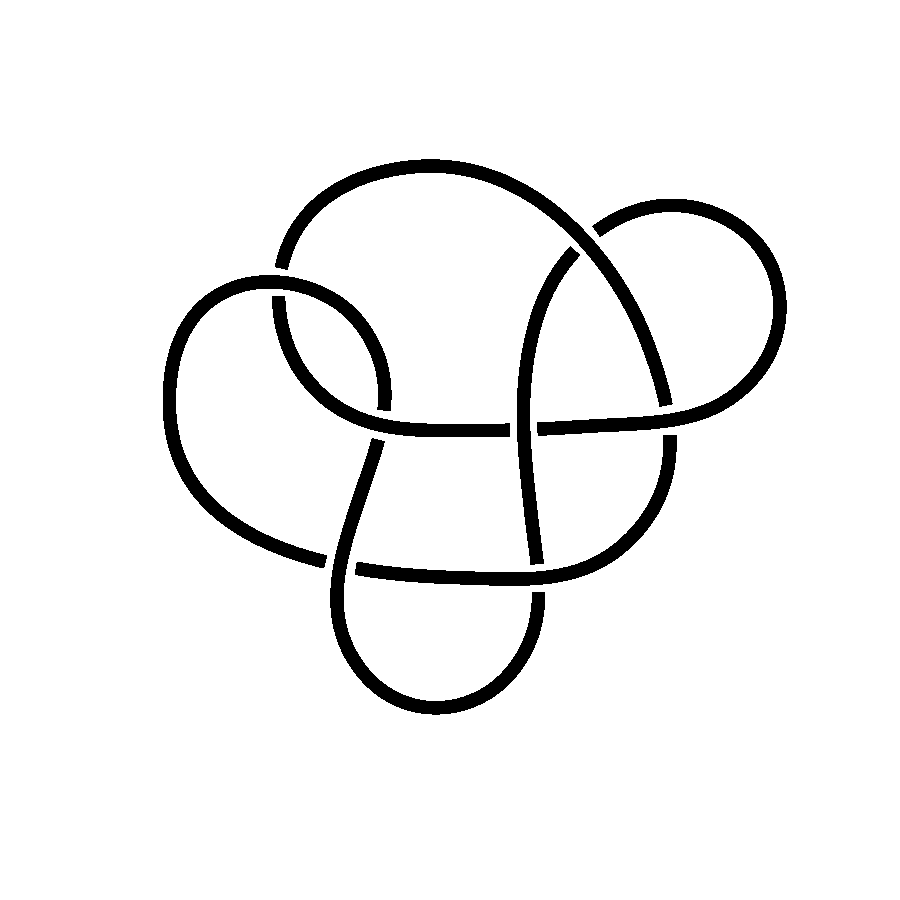
\includegraphics[scale = 0.9]{knot-009}% in vignettes/ directory
\caption{Knot $7_6$, post-optimization with breaks indicating
  \label{76_overunder}  underpassing strands}
\end{figure}

\subsection{Symmetry}

If a knot diagram can be drawn with a particular symmetry, one common
response is to demand that this symmetry be respected exactly.
Bosch~\cite{bosch2010}, for example, considered rotational symmetry to
be sufficiently important to impose five-fold rotational symmetry in
one of his works; similar comments apply to mirror symmetry.  Many of
the knots in Figure~\ref{knot_table} have an axis of symmetry, or
possess rotational symmetry; some have both and thus have a dihedral
symmetry group.  The package implements symmetry in a similar way to
that of Bosch~\cite{bosch2010}: one can impose these symmetry
relations on knots, and optimize the resulting symmetrical knot.

Minimizing the badness is not entirely straightforward on account of
the induced redundancy, which is characterized using a symmetry object
specific to the knot under consideration.  However, symmetry
constraints do reduce the dimensionality of the optimization problem.

I will consider the figure-of-eight knot~$4_1$ as an example.  Using
Figure~\ref{four_figure_8_knots}, top left, as reference, the
appropriate symmetry object is defined as follows:

\begin{verbatim}
> fig8 <- reader(system.file("4_1_first_draft.svg",package="knotR"))
> Mver8 <- matrix(c(
+     02,03,
+     09,07,
+     05,11,
+     10,06
+     ),ncol=2,byrow=TRUE)
> sym8 <- symmetry_object(fig8, Mver=Mver8, xver=8)
\end{verbatim}

(Matrix {\tt Mver8} specifies that nodes~2 and~3 are symmetric, as are
nodes~9 and~7, and so on; {\tt xver=8} forces node~8 to be on the axis
of symmetry).  The results are shown in
Figure~\ref{four_figure_8_knots}.  Note that $4_1$ may be rendered in
a form that has two mirror lines, and this is available in the package
as object {\tt k4\_1a}.

\begin{figure}[!tbp]
  \centering
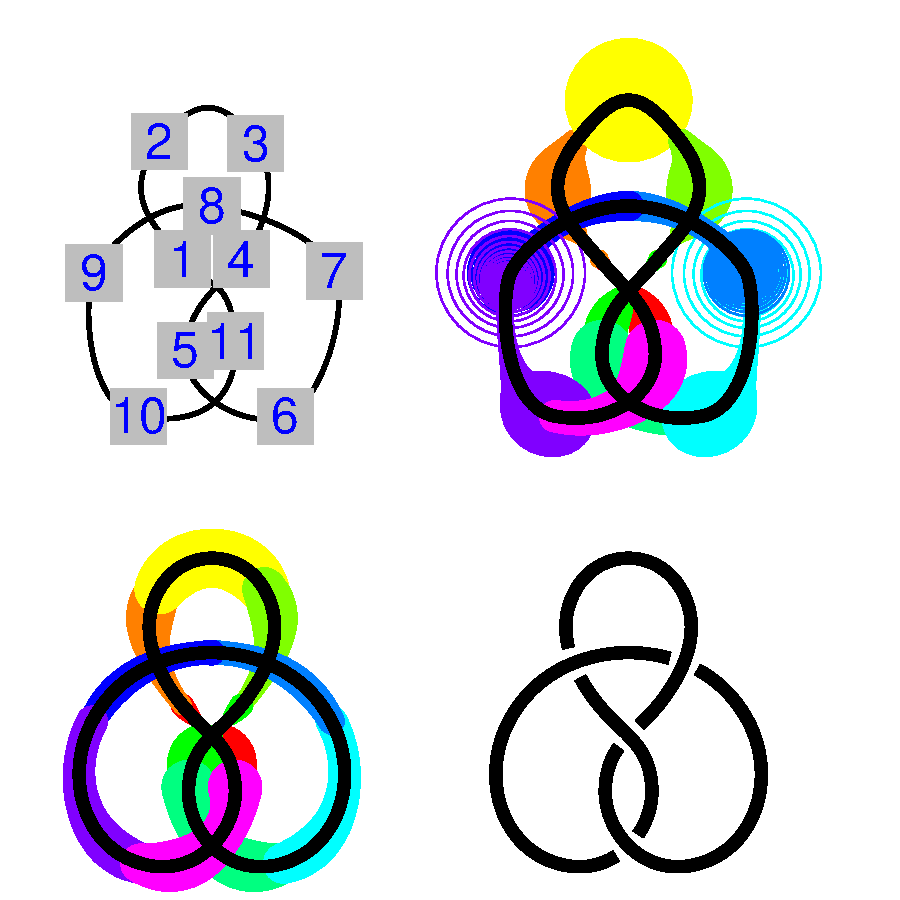
\includegraphics[width=11cm]{knot-four_figure_eight_knots}  % in vignettes/ directory
\caption{Figure eight knots drawn using different plotting methods.
  Top left, knot path with node numbers shown in order to facilitate
    \label{four_figure_8_knots} definition of the symmetry object; top
    right, result of symmetrizing the rough path; lower left, the
    optimized knot with imposed vertical symmetry, with curvature
    plotted; lower right, knot plotted with overstrand and understrand
    indicated using line breaks}
\end{figure}


\subsection{Rotational symmetry}

Consider knot~$5_1$. This knot has $D_5$ symmetry with five mirror
lines.  The package includes functionality to impose appropriate
symmetry constraints. Using Figure~\ref{k5_1_twoknots} as reference,
we have:

\begin{figure}[htbp]
  \begin{center}
\begin{verbatim}
> knotplot2(k5_1,node=TRUE,width=FALSE)
\end{verbatim}
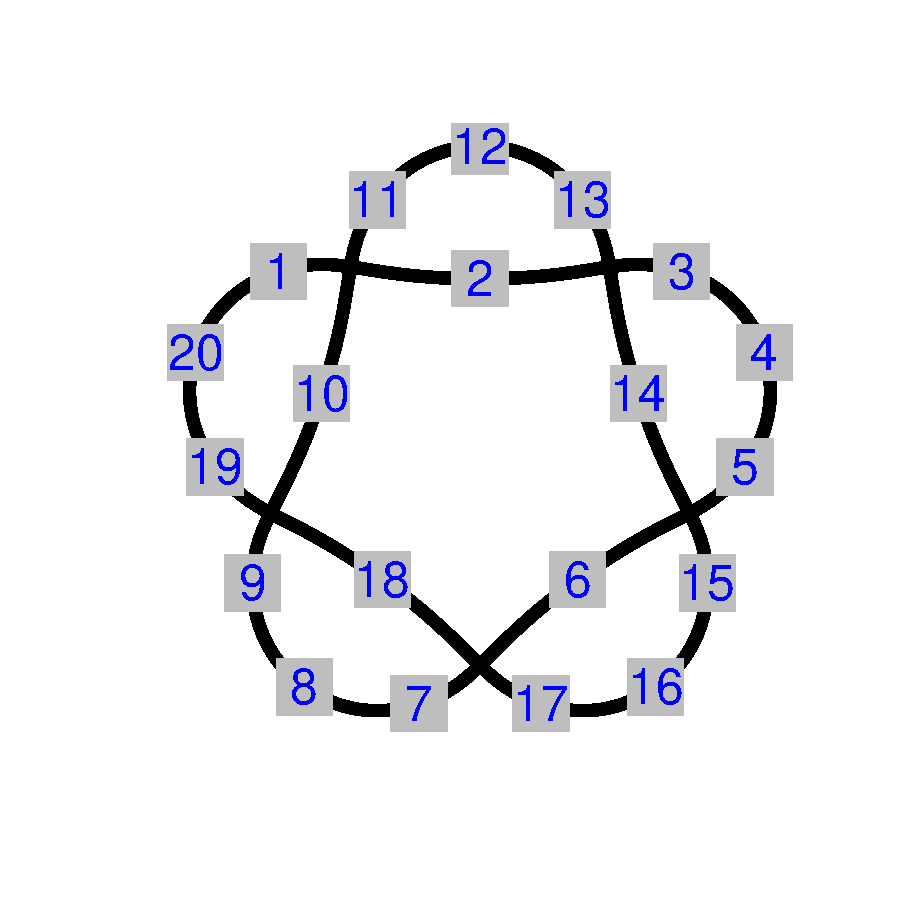
\includegraphics[width=11cm]{knot-k5_1}  % in vignettes/ directory
\caption{Knot $5_1$ \label{k5_1_twoknots} shown with node numbers}
  \end{center}
\end{figure}

\begin{verbatim}
> sym51 <- symmetry_object(k5_1,
+                          Mver = cbind(11,13),
+                          xver = c(2,12),
+                          Mrot = rbind(
+                              c(12,04,16,08,20),
+                              c(13,05,17,09,01),
+                              c(11,03,15,07,19),
+                              c(02,14,06,18,10)
+                          ))
\end{verbatim}

Thus, using the same notation as before, nodes~11 and~13 are
symmetrical about the vertical axis, nodes~2 and~12 are on the
vertical axis.  The {\tt Mrot} argument specifies sets of nodes that
map to themselves under rotation.  The top line of {\tt Mrot}
indicates that nodes 12, 4, 16, 8, and~20 are concyclic and indeed
from Figure~\ref{k5_1_twoknots} we see that these nodes are
constrained to lie on one of the five lines of symmetry, cutting it at
$90^\circ$.  An example of a knot with pure rotational symmetry,
rather than dihedral symmetry, is given in Figure~\ref{orn20}.

\subsection{Subjective \label{section_cca} choice for weighting}


One of the benefits of the {\tt knotR} software is that it allows the
relative importance of the different aspects of appearance to be
assessed.  In the package, the badness weightings may be altered
easily, and in this way we can investigate the visual impact of the
badness components.  The default weightings were originally chosen as
a bland compromise, but it is easy to place greater weight on one or
other component.  Figure~\ref{figure_cca} shows the same knot optimized
using different weightings; we see the effect of imposing right-angled
strand crossing angles on the remainder of the knot.  Readers will
have to judge for themselves which version they prefer.

\begin{figure}[htbp]
  \begin{center}
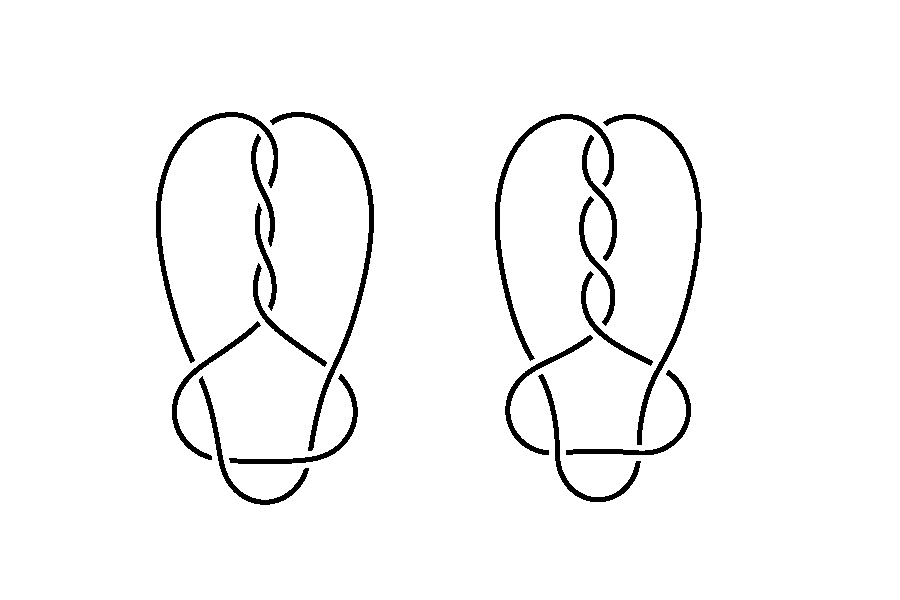
\includegraphics[width=13cm]{compare_crossing_angles}  % created by
                                                       % inst/knotter.R
\caption{Comparison between optimized knot projections for $8_3$
  \label{figure_cca} using different  badness weightings.  On the
  left we see the default knot, and on the right we see the result of
  increasing the angle-crossing penalty by a factor of 100,
  effectively forcing all strand crossing angles to be $\pi/2$.  Which
  one is preferable is, of course, a subjective choice}
  \end{center}
\end{figure}


\section{Conclusions and further work}

The {\tt knotR} package allows the user to create rough diagrams of
knots using the inkscape suite of software, and subsequently polish up
such diagrams in terms of a customizable objective function using
numerical optimization techniques.  The software makes a large number
of pleasing knot diagrams available to the community under the GPL.

One suggestion is that the software might be used in preference tests.
Subjects might be asked to state which of two knots [e.g. the two
  shown in Figure~\ref{figure_cca}] they find more attractive.  This
might allow us to make inferences about the mathematical basis for
aesthetics of knot diagrams---or perhaps to quantify some features of
subjective decision-making.

Further work might include adding functionality to deal with links,
although this is not straightforward, and a brief discussion is given
in Appendix B.

In the broader context of optimisation in art, we observe that
numerical optimisation techniques can produce aesthetically pleasing
results, an observation that might find uptake by graphic artists.
Indeed, one could argue that real art lies in the capturing of
mathematical formulations of aesthetics.

\clearpage
\section{Gallery}

There now follows a selection of pleasing knot diagrams taken from
datasets provided with the package, illustrating the relative ease
with which knot diagrams may be created and optimized.
Figure~\ref{two_trefoil_knots} shows and compares two plausible
schemes for rendering a trefoil: optimized as per the {\tt knotR}
package techniques documented here; compared with a trefoil knot
constructed from arcs of circles constrained to cross at right angles.
In the circular-arc trefoil, the strands exert a couple but no force
on one another.  Mirror symmetry and threefold rotational symmetry are
imposed.  Elementary trigonometry shows that the radii of the inner
and outer loops are $\operatorname{cosec}(\pi/12)=\sqrt{6}+\sqrt{2}$
and $\sec(\pi/12)=\sqrt{6}-\sqrt{2}$ respectively.  We see the
disadvantages of placing nodes at crossing points.

Figure~\ref{perko_AB} shows two
forms of a 10-crossing knot once erroneously considered to be
topologically distinct; figure~\ref{orn20} shows an ornamental knot
with exact five-fold symmetry (but not dihedral symmetry); and
figure~\ref{all8} shows all prime knots with eight or fewer crossings,
following Rolfsen~\cite{rolfsen1976}.  The package includes all knots
to nine crossings.

\begin{figure}[h]
  \centering  
  % To create file "two_trefoil_knots_post_inkscape.pdf" (which is
  % stored on the repo), run knotter.R, which makes (among other
  % things) two_trefoil_knots.pdf.  Edit this in inkscape [make a
  % mirror image, then change the colours and finally use the raise
  % and lower tools to put everything in the right order]
    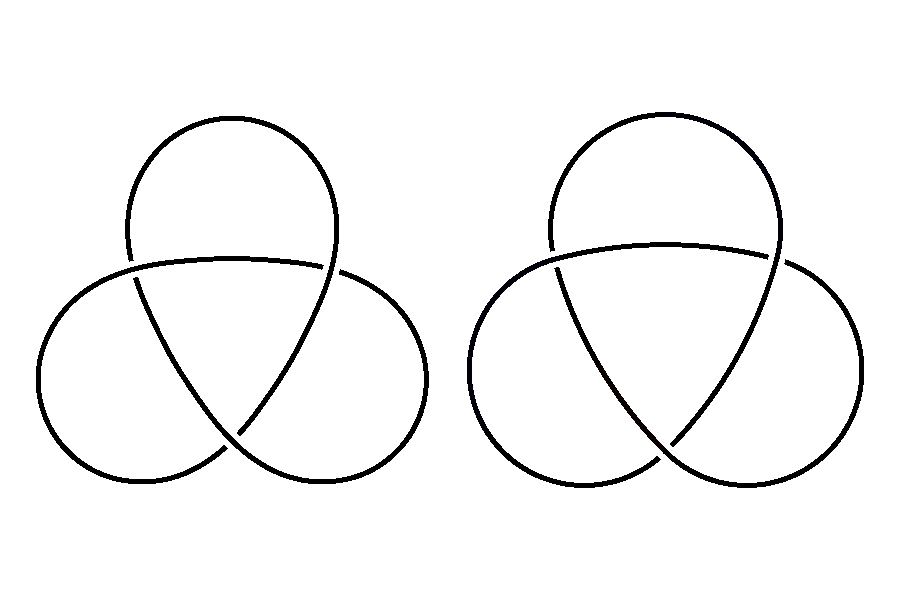
\includegraphics[width=10cm]{two_trefoil_knots_post_inkscape.pdf}
    \caption{Two trefoil \label{two_trefoil_knots} knots.  Left,
      optimized as per the {\tt knotR} package techniques documented
      here; right, constructed from arcs of circles constrained to
      cross at right angles.    On the right, the curvature
      has a displeasing discontinuity at a node which interrupts
      the visual continuity there, especially the understrand}
\end{figure}

\begin{figure}[htbp]
  \begin{center}
\begin{verbatim}
par(mfcol=1:2)
knotplot(perko_A)
knotplot(perko_B)
\end{verbatim}
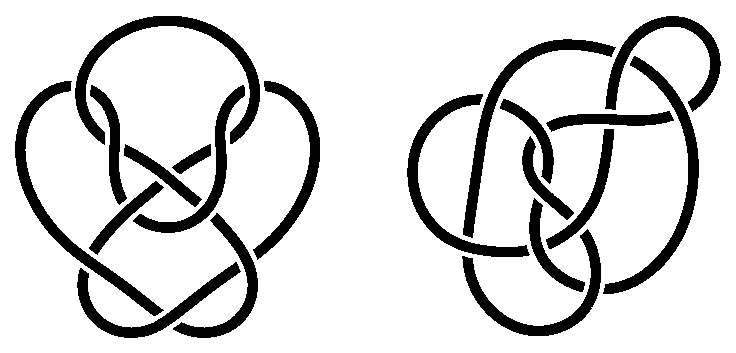
\includegraphics[width=11cm]{knot-perko_A_and_B}  % in vignettes/ directory
\caption{Two representations of knot~$10_{125}$, known as the 
  \label{perko_AB}  Perko Pair.  The software requires the user to
  specify the symmetry (mirror or rotational) of a knot projection and
  has no notion of topological invariance of a knot}
  \end{center}
\end{figure}

\begin{figure}[htbp]
  \begin{center}
\begin{verbatim}
> knotplot(ornamental20,gap=15)
\end{verbatim}
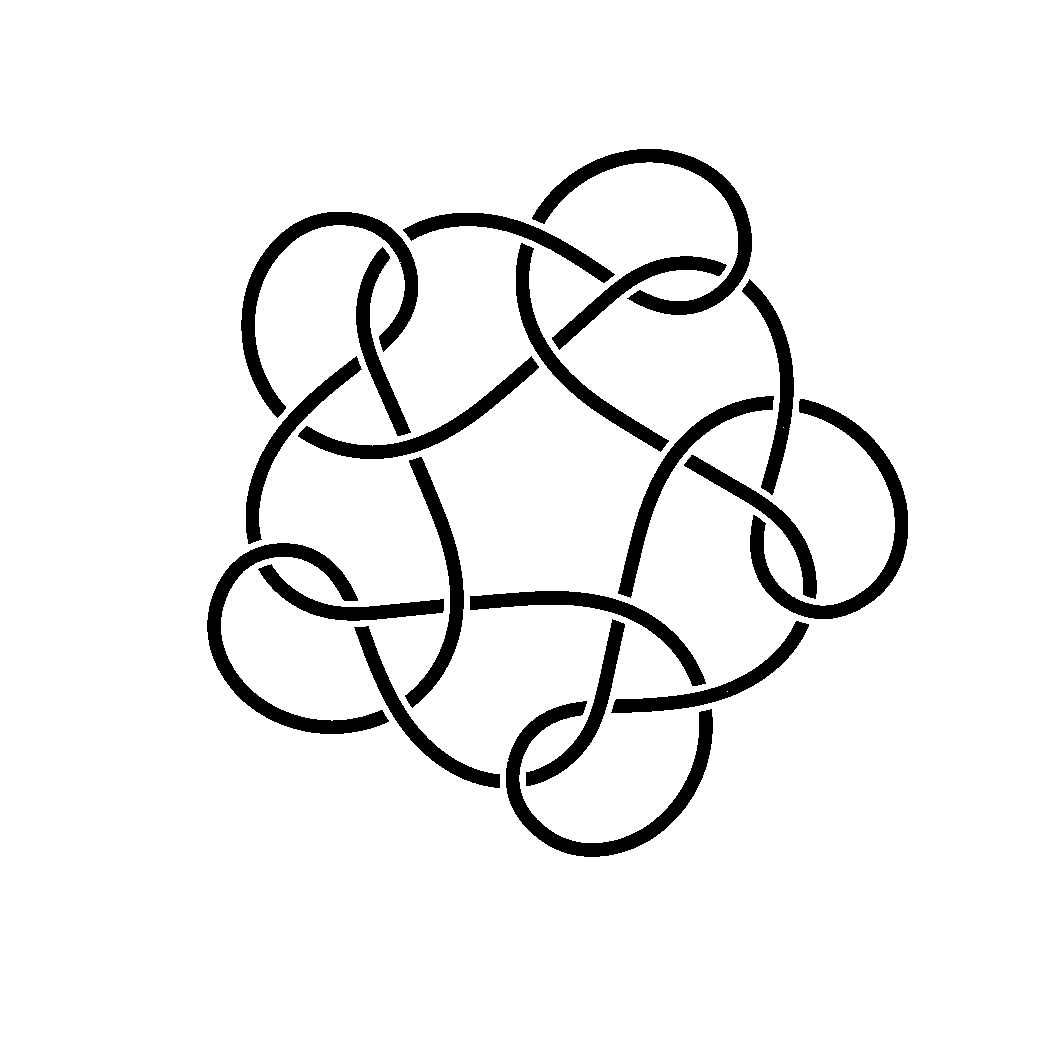
\includegraphics[width=11cm]{knot-ornamental} % in vignettes/ directory
\caption{An ornamental knot exhibiting fivefold
  rotational \label{orn20} symmetry $C_5$; note the absence of mirror
  symmetry which would impose $D_5$}
  \end{center}
\end{figure}

\begin{figure}[htbp]
  \begin{center}
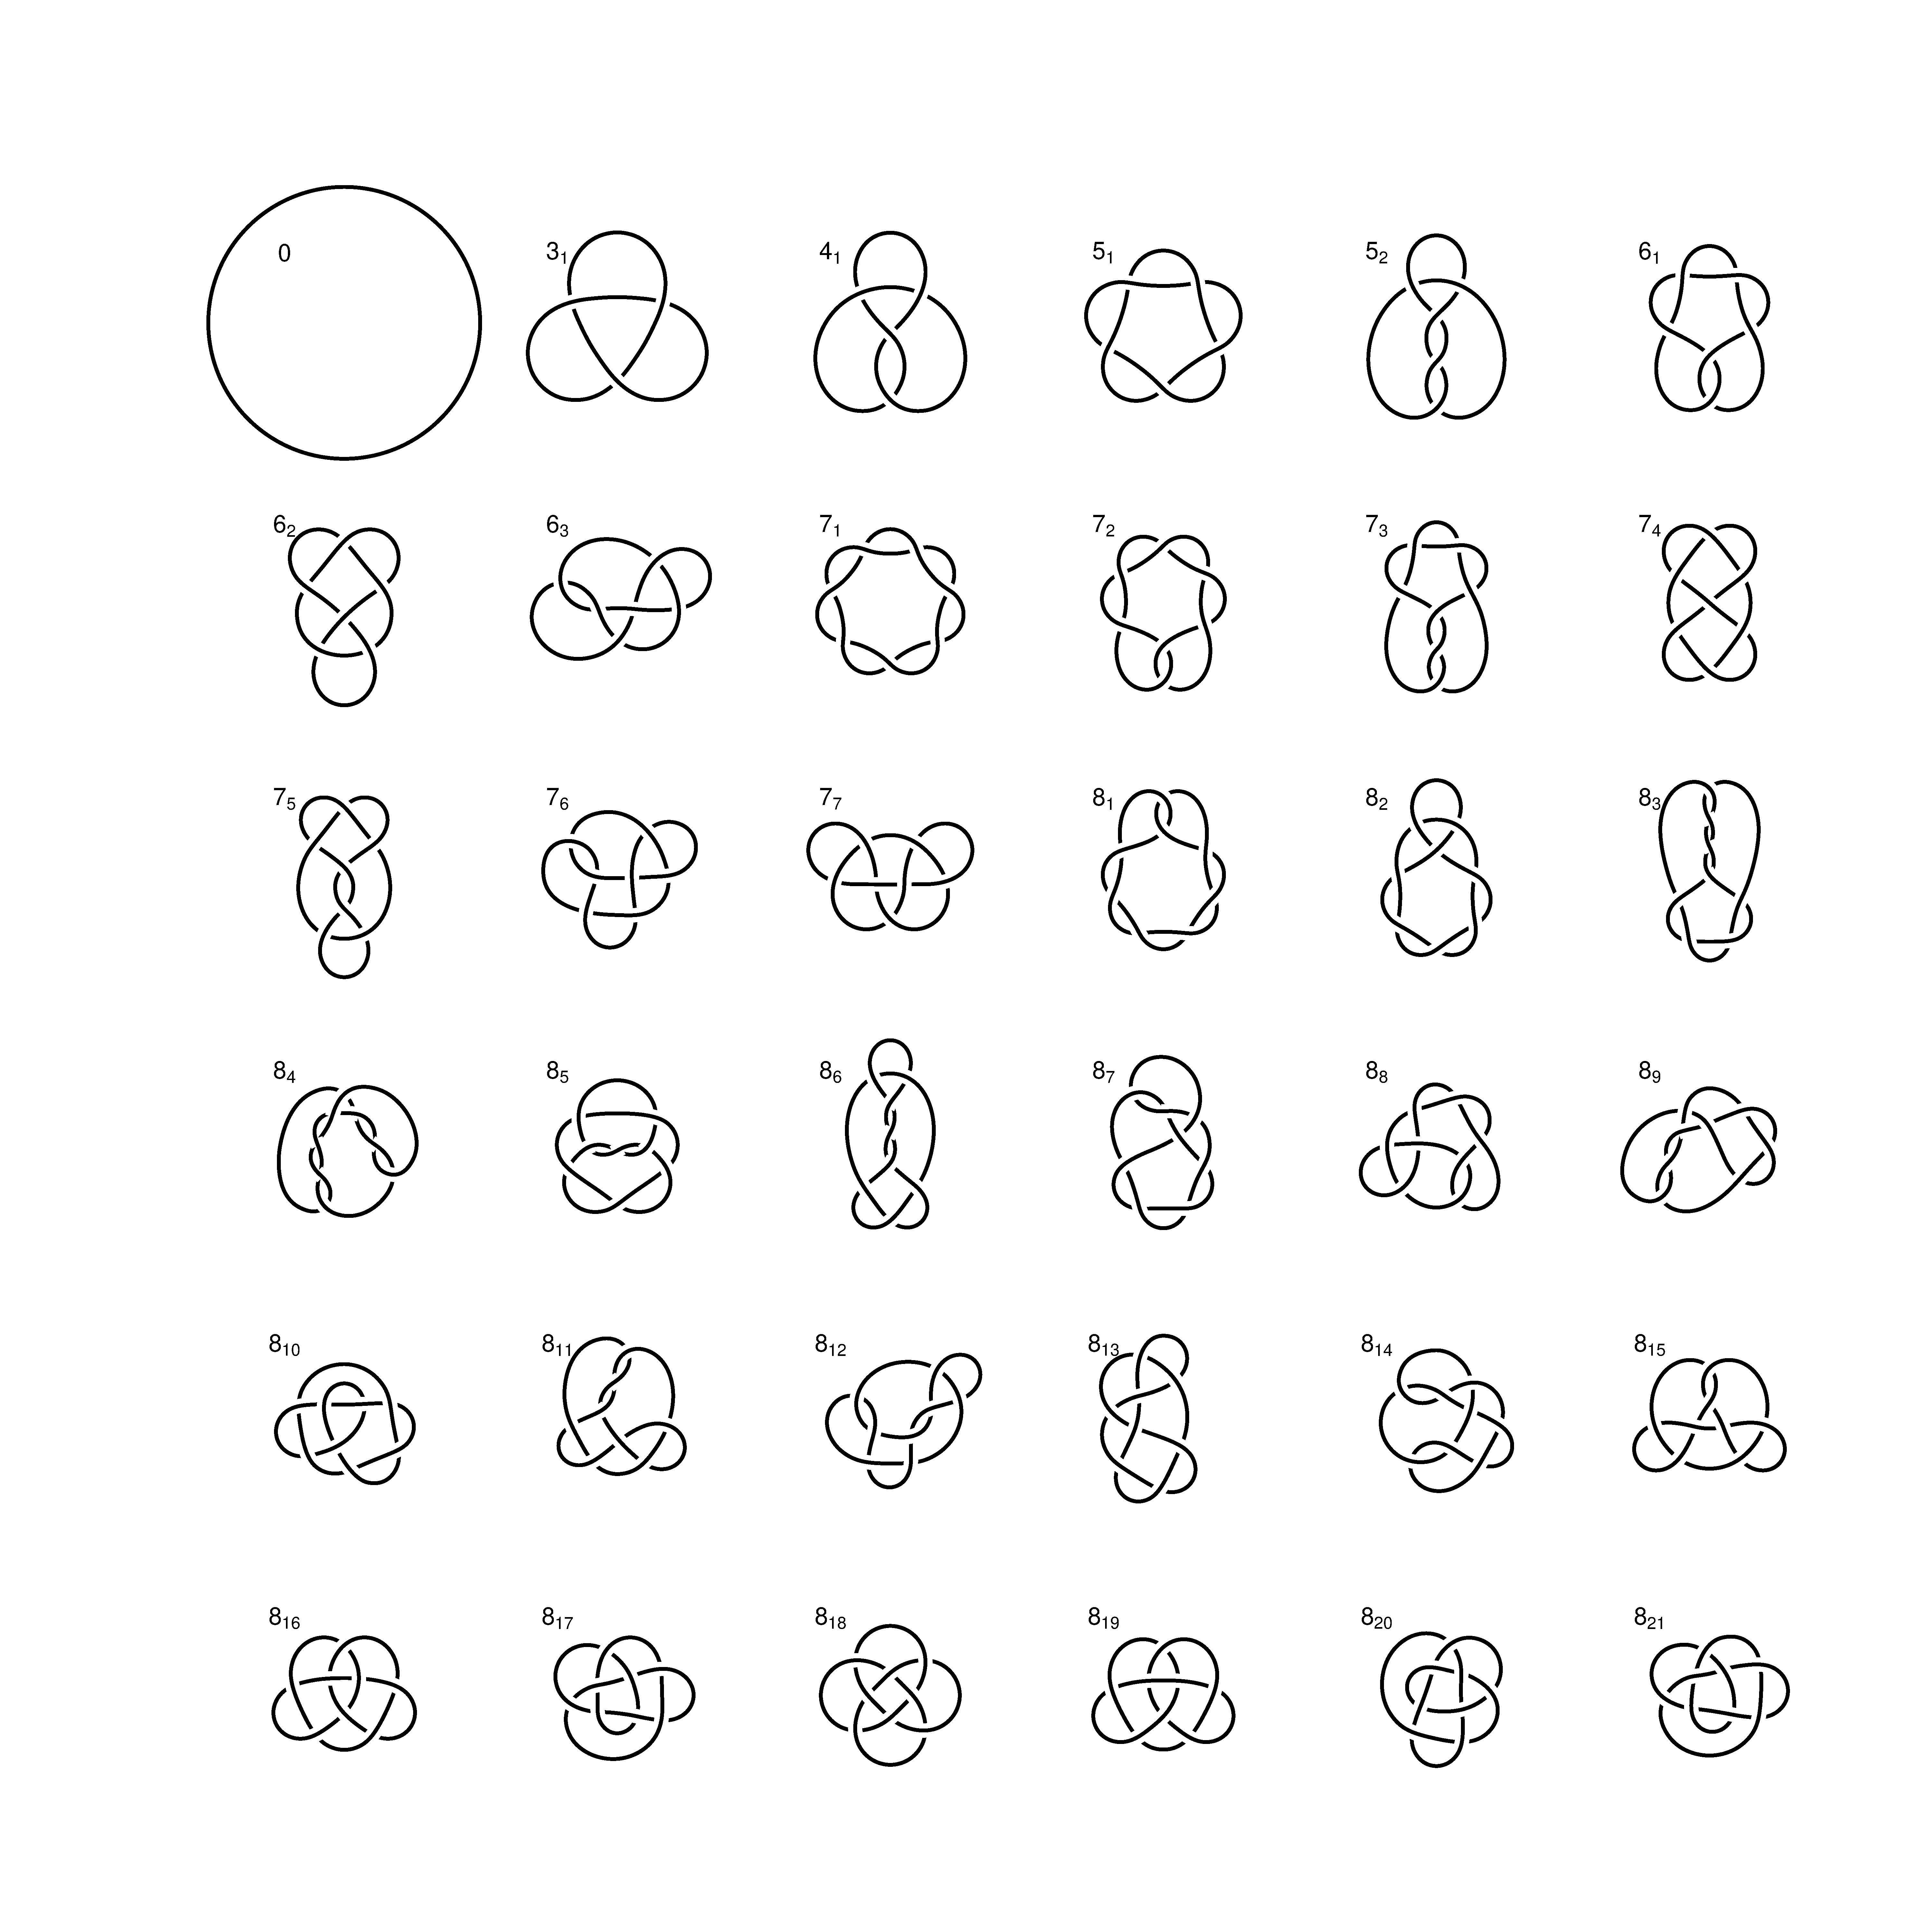
\includegraphics[width=13cm]{knots_to_8crossings}  % created by inst/knotter.R
\caption{All \label{all8} prime knots with 8 or fewer crossings,
  notation following Rolfsen~\cite{rolfsen1976}.  Here, the penalty
  for crossing angles departing from $90^\circ$ is relatively light
  and so knot $8_3$, for example, matches the left diagram of
  Figure~\ref{figure_cca}, rather than the right}
  \end{center}
\end{figure}

\bibliography{knot}
\bibliographystyle{unsrt}

\clearpage
\section*{Appendix A: details and motivation for the badness functions}

There follows a more detailed description and motivation for various
metrics used to evaluate knot diagrams in the package.

\begin{description}
\item[{\tt total\_crossing\_potential\_energy()}] The idea is to make
  the crossing points attract one another as if they are
  gravitationally active objects; metric measured by their mutual
  potential energy.  If crossing point $i$ is at position ${\mathbf
    p}_i$ we have $\sum_{i\neq j}\left|{\mathbf p}_i-{\mathbf
    p}_j\right|^{2}$.  The idea is to encourage more compact
  configurations rather than long skinny ones.
\item[{\tt node\_crossing\_badness()}] Here we make the crossing
  points {\em repel} one another, as though they are all charged
  objects (with the same sign).  The idea is to spread out the nodes
  so no two nodes are too close together.  If crossing point $i$ is at
  position ${\mathbf p}_i$ we have $\sum_{i\neq j}\left|{\mathbf
    p}_i-{\mathbf p}_j\right|^{-1}$.  The length scale for this
  repulsion is smaller than that of the attractive term above.  The
  overall potential thus resembles that sometimes seen in atomic
  physics when considering the hydrogen molecule $H_2$: the two
  protons attract one another when distant, but repel when closer.  In
  the package, the intent is for this optimal distance to be a shallow
  minimum and the optimization routine is free to adjust within a wide
  range.
\item[{\tt total\_crossing\_angles()}] Here we wish to punish
  configurations with strands that cross at acute angles.  If crossing
  point $i$ has crossing angle $\theta_i$ the metric is
  $\sum_i\left(\cos\theta_i\right)^2$.
\item[{\tt total\_bending\_energy()}] The idea is for the strands to
  preferentially follow elastica curves, as in elementary (nonlinear)
  beam theory.  From differential geometry, the Euler elastica
  potential energy is $\int\kappa(s)^2\,ds$.  In the package, this is
  calculated numerically for each strand and the total returned.
\item[{\tt total\_string\_length()}] The length is just $\int ds$, with a
  nominal value of 5000 (which value is about right for a printed
  copy).
\item[{\tt midpoint\_badness()}] The idea is to suppress strands with
  crossing points too close to the endpoint nodes.  For each crossing
  point $c_{ij}$ of strand $i$ with strand $j$, we calculate the arc
  length $\int_{s=0}^{c_{ij}}\,ds$ from the node to each crossing
  point and normalize with the strand length $\int\,ds$.  We reward
  configurations with normalized crossing point arc lengths that are
  close to $1/2$.  Note that this particular metric is not independent
  of the total crossing potential energy metric.
\item[{\tt curvature\_switching\_badness()}] Here the problem is knots
  which should have either all their strands curving to the left, or
  all to the right; the signed curvature should be everywhere the same
  sign (the canonical example would be $8_{18}$ which in earlier
  versions of the software had ugly changes of curvature).  We impose
  a fixed penalty for any knot with more than one sign.
\item[{\tt curvature\_consecutive\_segment\_switching\_badness()}] We
  wish to discourage configurations in which curvature undergoes a
  sudden change at a node.  The value for a single (Bezier) node is
  simply $\left(\delta\kappa\right)^2$, and the penalty for a given
  configuration is the sum of the values for each node.  See
  Figure~\ref{two_trefoil_knots} for motivation and discussion.
\item[{\tt non\_crossing\_strand\_close\_approach\_badness()}] Here
  the idea is to prevent non-intersecting strands from approaching one
  another too closely.  Quite apart from aesthetic considerations,
  this metric prevents the creation of new spurious nodes that would
  disrupt the optimization routines.
\end{description}

\section*{Appendix B: some reflections on links}

Further work might include functionality to deal with links.  Much of
the required functionality is (in principle) already present in the
software.  Each component would have its own badness, and in addition
there would be $n(n-1)/2$ inter-component interaction terms measuring
features such as closeness between non-intersecting strands of
different components.  However, the implementation of such
functionality is not straightforward and several problems stand out.
Firstly, dealing with inter-component intersection points is
difficult.  Currently, crossing points are represented as a
(symmetrical) Boolean matrix with rows and columns corresponding to
strands, and entry $(i,j)$ being whether strand $i$ intersects with
strand $j$.  The link generalization would be a symmetric matrix with
entries that are themselves intersection matrices: an object with four
indices and entry $(i,j,k,l)$ indicating whether strand $j$ of
component $i$ intersects strand $l$ of component $k$.  Such objects
are unwieldy to work with and are typically difficult to manipulate.
Secondly, the imposition of symmetry is not straightforward in the
case of links: one might desire that certain components of a link have
a particular kind of symmetry and others to have a different kind (or
no!) symmetry.  Further, one unexpectedly difficult problem was
dealing with a subset of components that individually possess no
symmetry but collectively possess mirror (or rotational) symmetry.
Even the simplest links, as in Figure~\ref{thistlethwaite}, can be
problematic.  Consider Thistlethwaite's L4a1, for example: one would
expect the two components to be identical except for a 90-degree
rotation, and implementing this in the context of the package does not
seem to be at all easy.  In general, new badnesses would be needed.
Further, in L7a1, the smaller component should be not only as circular
as possible (?), but also one might desire the overall length to be
smaller than that of the other component.  It would be reasonable to
conclude that dealing with links might be possible in principle but,
due to a number of technical and mathematical reasons, considerably
harder than the single-component links considered here.


\begin{figure}[htbp]
  \begin{center}
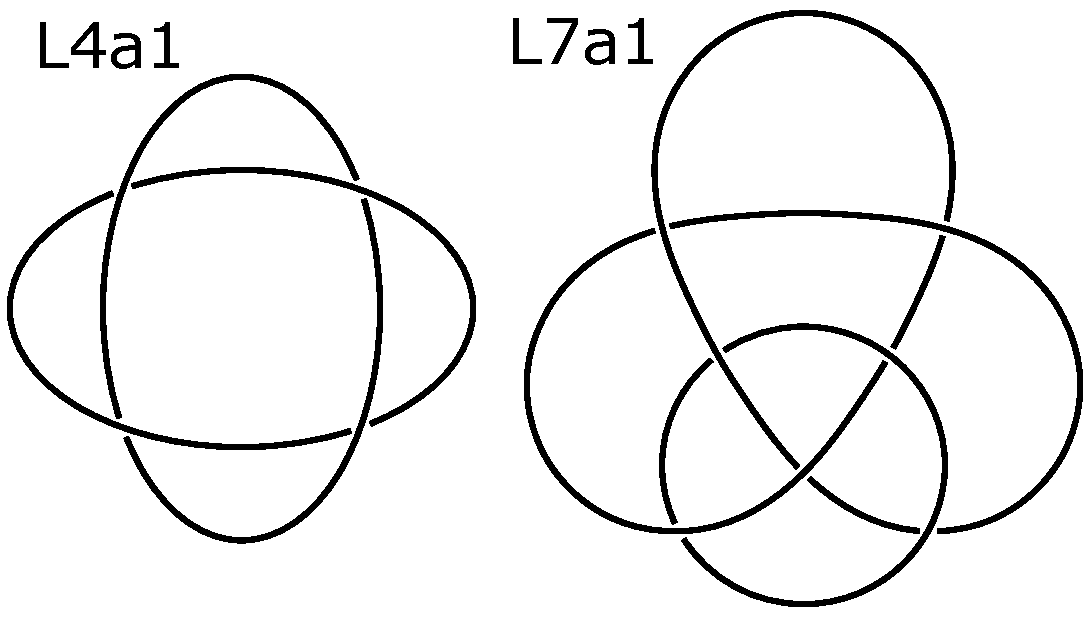
\includegraphics[width=7cm]{L4a1_L7a1}  % made by exporting L4a1_L7a1.svg as PDF
\caption{Two links \label{thistlethwaite} taken from the
  Thistlethwaite link table~\cite{hoste1998}.  These are produced
  directly with inkscape and are not optimized}
  \end{center}
\end{figure}





\end{document}

